% Options for packages loaded elsewhere
\PassOptionsToPackage{unicode}{hyperref}
\PassOptionsToPackage{hyphens}{url}
%
\documentclass[
  ignorenonframetext,
]{beamer}
\usepackage{pgfpages}
\setbeamertemplate{caption}[numbered]
\setbeamertemplate{caption label separator}{: }
\setbeamercolor{caption name}{fg=normal text.fg}
\beamertemplatenavigationsymbolshorizontal
% Prevent slide breaks in the middle of a paragraph
\widowpenalties 1 10000
\raggedbottom
\setbeamertemplate{part page}{
  \centering
  \begin{beamercolorbox}[sep=16pt,center]{part title}
    \usebeamerfont{part title}\insertpart\par
  \end{beamercolorbox}
}
\setbeamertemplate{section page}{
  \centering
  \begin{beamercolorbox}[sep=12pt,center]{part title}
    \usebeamerfont{section title}\insertsection\par
  \end{beamercolorbox}
}
\setbeamertemplate{subsection page}{
  \centering
  \begin{beamercolorbox}[sep=8pt,center]{part title}
    \usebeamerfont{subsection title}\insertsubsection\par
  \end{beamercolorbox}
}
\AtBeginPart{
  \frame{\partpage}
}
\AtBeginSection{
  \ifbibliography
  \else
    \frame{\sectionpage}
  \fi
}
\AtBeginSubsection{
  \frame{\subsectionpage}
}

\usepackage{amsmath,amssymb}
\usepackage{iftex}
\ifPDFTeX
  \usepackage[T1]{fontenc}
  \usepackage[utf8]{inputenc}
  \usepackage{textcomp} % provide euro and other symbols
\else % if luatex or xetex
  \usepackage{unicode-math}
  \defaultfontfeatures{Scale=MatchLowercase}
  \defaultfontfeatures[\rmfamily]{Ligatures=TeX,Scale=1}
\fi
\usepackage{lmodern}
\usetheme[]{AnnArbor}
\ifPDFTeX\else  
    % xetex/luatex font selection
\fi
% Use upquote if available, for straight quotes in verbatim environments
\IfFileExists{upquote.sty}{\usepackage{upquote}}{}
\IfFileExists{microtype.sty}{% use microtype if available
  \usepackage[]{microtype}
  \UseMicrotypeSet[protrusion]{basicmath} % disable protrusion for tt fonts
}{}
\makeatletter
\@ifundefined{KOMAClassName}{% if non-KOMA class
  \IfFileExists{parskip.sty}{%
    \usepackage{parskip}
  }{% else
    \setlength{\parindent}{0pt}
    \setlength{\parskip}{6pt plus 2pt minus 1pt}}
}{% if KOMA class
  \KOMAoptions{parskip=half}}
\makeatother
\usepackage{xcolor}
\newif\ifbibliography
\setlength{\emergencystretch}{3em} % prevent overfull lines
\setcounter{secnumdepth}{-\maxdimen} % remove section numbering

\usepackage{color}
\usepackage{fancyvrb}
\newcommand{\VerbBar}{|}
\newcommand{\VERB}{\Verb[commandchars=\\\{\}]}
\DefineVerbatimEnvironment{Highlighting}{Verbatim}{commandchars=\\\{\}}
% Add ',fontsize=\small' for more characters per line
\usepackage{framed}
\definecolor{shadecolor}{RGB}{241,243,245}
\newenvironment{Shaded}{\begin{snugshade}}{\end{snugshade}}
\newcommand{\AlertTok}[1]{\textcolor[rgb]{0.68,0.00,0.00}{#1}}
\newcommand{\AnnotationTok}[1]{\textcolor[rgb]{0.37,0.37,0.37}{#1}}
\newcommand{\AttributeTok}[1]{\textcolor[rgb]{0.40,0.45,0.13}{#1}}
\newcommand{\BaseNTok}[1]{\textcolor[rgb]{0.68,0.00,0.00}{#1}}
\newcommand{\BuiltInTok}[1]{\textcolor[rgb]{0.00,0.23,0.31}{#1}}
\newcommand{\CharTok}[1]{\textcolor[rgb]{0.13,0.47,0.30}{#1}}
\newcommand{\CommentTok}[1]{\textcolor[rgb]{0.37,0.37,0.37}{#1}}
\newcommand{\CommentVarTok}[1]{\textcolor[rgb]{0.37,0.37,0.37}{\textit{#1}}}
\newcommand{\ConstantTok}[1]{\textcolor[rgb]{0.56,0.35,0.01}{#1}}
\newcommand{\ControlFlowTok}[1]{\textcolor[rgb]{0.00,0.23,0.31}{#1}}
\newcommand{\DataTypeTok}[1]{\textcolor[rgb]{0.68,0.00,0.00}{#1}}
\newcommand{\DecValTok}[1]{\textcolor[rgb]{0.68,0.00,0.00}{#1}}
\newcommand{\DocumentationTok}[1]{\textcolor[rgb]{0.37,0.37,0.37}{\textit{#1}}}
\newcommand{\ErrorTok}[1]{\textcolor[rgb]{0.68,0.00,0.00}{#1}}
\newcommand{\ExtensionTok}[1]{\textcolor[rgb]{0.00,0.23,0.31}{#1}}
\newcommand{\FloatTok}[1]{\textcolor[rgb]{0.68,0.00,0.00}{#1}}
\newcommand{\FunctionTok}[1]{\textcolor[rgb]{0.28,0.35,0.67}{#1}}
\newcommand{\ImportTok}[1]{\textcolor[rgb]{0.00,0.46,0.62}{#1}}
\newcommand{\InformationTok}[1]{\textcolor[rgb]{0.37,0.37,0.37}{#1}}
\newcommand{\KeywordTok}[1]{\textcolor[rgb]{0.00,0.23,0.31}{#1}}
\newcommand{\NormalTok}[1]{\textcolor[rgb]{0.00,0.23,0.31}{#1}}
\newcommand{\OperatorTok}[1]{\textcolor[rgb]{0.37,0.37,0.37}{#1}}
\newcommand{\OtherTok}[1]{\textcolor[rgb]{0.00,0.23,0.31}{#1}}
\newcommand{\PreprocessorTok}[1]{\textcolor[rgb]{0.68,0.00,0.00}{#1}}
\newcommand{\RegionMarkerTok}[1]{\textcolor[rgb]{0.00,0.23,0.31}{#1}}
\newcommand{\SpecialCharTok}[1]{\textcolor[rgb]{0.37,0.37,0.37}{#1}}
\newcommand{\SpecialStringTok}[1]{\textcolor[rgb]{0.13,0.47,0.30}{#1}}
\newcommand{\StringTok}[1]{\textcolor[rgb]{0.13,0.47,0.30}{#1}}
\newcommand{\VariableTok}[1]{\textcolor[rgb]{0.07,0.07,0.07}{#1}}
\newcommand{\VerbatimStringTok}[1]{\textcolor[rgb]{0.13,0.47,0.30}{#1}}
\newcommand{\WarningTok}[1]{\textcolor[rgb]{0.37,0.37,0.37}{\textit{#1}}}

\providecommand{\tightlist}{%
  \setlength{\itemsep}{0pt}\setlength{\parskip}{0pt}}\usepackage{longtable,booktabs,array}
\usepackage{calc} % for calculating minipage widths
\usepackage{caption}
% Make caption package work with longtable
\makeatletter
\def\fnum@table{\tablename~\thetable}
\makeatother
\usepackage{graphicx}
\makeatletter
\def\maxwidth{\ifdim\Gin@nat@width>\linewidth\linewidth\else\Gin@nat@width\fi}
\def\maxheight{\ifdim\Gin@nat@height>\textheight\textheight\else\Gin@nat@height\fi}
\makeatother
% Scale images if necessary, so that they will not overflow the page
% margins by default, and it is still possible to overwrite the defaults
% using explicit options in \includegraphics[width, height, ...]{}
\setkeys{Gin}{width=\maxwidth,height=\maxheight,keepaspectratio}
% Set default figure placement to htbp
\makeatletter
\def\fps@figure{htbp}
\makeatother

\titlegraphic{
\includegraphics[width=0.4\paperwidth]{logos.png}}
\pgfdeclareimage[height=.75cm]{logoAFA}{logos.png}
\logo{\pgfuseimage{logoAFA}}
\makeatletter
\makeatother
\makeatletter
\makeatother
\makeatletter
\@ifpackageloaded{caption}{}{\usepackage{caption}}
\AtBeginDocument{%
\ifdefined\contentsname
  \renewcommand*\contentsname{Table of contents}
\else
  \newcommand\contentsname{Table of contents}
\fi
\ifdefined\listfigurename
  \renewcommand*\listfigurename{List of Figures}
\else
  \newcommand\listfigurename{List of Figures}
\fi
\ifdefined\listtablename
  \renewcommand*\listtablename{List of Tables}
\else
  \newcommand\listtablename{List of Tables}
\fi
\ifdefined\figurename
  \renewcommand*\figurename{Figure}
\else
  \newcommand\figurename{Figure}
\fi
\ifdefined\tablename
  \renewcommand*\tablename{Table}
\else
  \newcommand\tablename{Table}
\fi
}
\@ifpackageloaded{float}{}{\usepackage{float}}
\floatstyle{ruled}
\@ifundefined{c@chapter}{\newfloat{codelisting}{h}{lop}}{\newfloat{codelisting}{h}{lop}[chapter]}
\floatname{codelisting}{Listing}
\newcommand*\listoflistings{\listof{codelisting}{List of Listings}}
\makeatother
\makeatletter
\@ifpackageloaded{caption}{}{\usepackage{caption}}
\@ifpackageloaded{subcaption}{}{\usepackage{subcaption}}
\makeatother
\makeatletter
\@ifpackageloaded{tcolorbox}{}{\usepackage[skins,breakable]{tcolorbox}}
\makeatother
\makeatletter
\@ifundefined{shadecolor}{\definecolor{shadecolor}{rgb}{.97, .97, .97}}
\makeatother
\makeatletter
\makeatother
\makeatletter
\makeatother
\ifLuaTeX
  \usepackage{selnolig}  % disable illegal ligatures
\fi
\IfFileExists{bookmark.sty}{\usepackage{bookmark}}{\usepackage{hyperref}}
\IfFileExists{xurl.sty}{\usepackage{xurl}}{} % add URL line breaks if available
\urlstyle{same} % disable monospaced font for URLs
\hypersetup{
  pdftitle={Mandalas},
  pdfauthor={Profa. Dra. Luciane, Prof.~Dr.~João Paulo, Prof.~Dr.~Orlando e Prof.~Dr.~Ariel},
  hidelinks,
  pdfcreator={LaTeX via pandoc}}

\title{Mandalas}
\subtitle{ uma Abordagem para Desenvolver Habilidades Humanas com R}
\author{Profa. Dra. Luciane, Prof.~Dr.~João Paulo, Prof.~Dr.~Orlando e
Prof.~Dr.~Ariel}
\date{2023-01-01}
\institute{Academia da Força Aérea/ Universidade Federal Fluminense}

\begin{document}
\frame{\titlepage}
\ifdefined\Shaded\renewenvironment{Shaded}{\begin{tcolorbox}[breakable, borderline west={3pt}{0pt}{shadecolor}, interior hidden, frame hidden, sharp corners, enhanced, boxrule=0pt]}{\end{tcolorbox}}\fi

\begin{frame}[fragile]
\begin{block}{Quarto}
\protect\hypertarget{quarto}{}
Quarto enables you to weave together content and executable code into a
finished presentation. To learn more about Quarto presentations see
\url{https://quarto.org/docs/presentations/}.
\end{block}

\begin{block}{Bullets}
\protect\hypertarget{bullets}{}
When you click the \textbf{Render} button a document will be generated
that includes:

\begin{itemize}
\tightlist
\item
  Content authored with markdown
\item
  Output from executable code
\end{itemize}
\end{block}

\begin{block}{Code}
\protect\hypertarget{code}{}
When you click the \textbf{Render} button a presentation will be
generated that includes both content and the output of embedded code.
You can embed code like this:

\begin{verbatim}
[1] 2
\end{verbatim}
\end{block}
\end{frame}

\begin{frame}{guión de presentación}
\protect\hypertarget{guiuxf3n-de-presentaciuxf3n}{}
\begin{itemize}
\tightlist
\item
  Que hacemos
\item
  Introducción

  \begin{itemize}
  \tightlist
  \item
    Valores Humanos x Habilidades Humanas x R x Mandalas
  \end{itemize}
\item
  Objetivos
\item
  Conceptos matemáticos
\item
  Actividades
\item
  Resultados
\item
  Consideraciones finales
\end{itemize}
\end{frame}

\begin{frame}{Difusión de R en la comunidad}
\protect\hypertarget{difusiuxf3n-de-r-en-la-comunidad}{}
Selección de Libros, Encuentros y Seminarios

\begin{figure}

{\centering 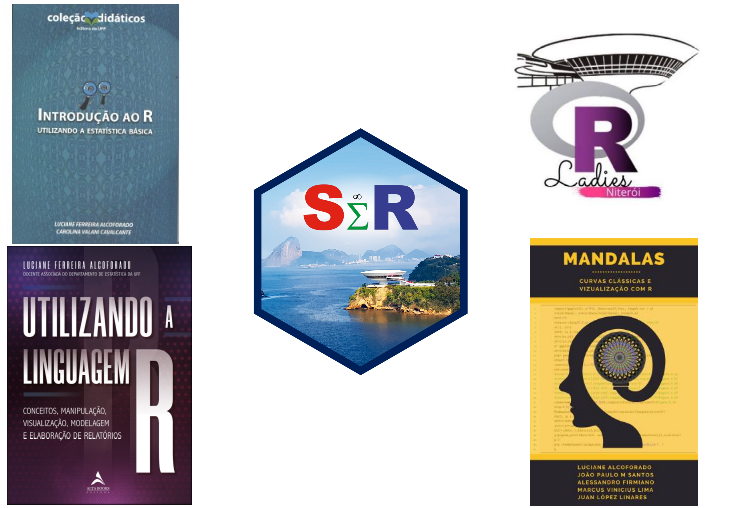
\includegraphics[width=1.5625in,height=\textheight]{FigurasLatinR2023/Introducao.png}

}

\end{figure}
\end{frame}

\begin{frame}{Libro Abierto}
\protect\hypertarget{libro-abierto}{}
\url{https://www.livrosabertos.sibi.usp.br/portaldelivrosUSP/catalog/book/1017}

\begin{figure}

{\centering 
\includegraphics[width=0.625in,height=\textheight]{FigurasLatinR2023/QRCODE_livro.png}

}

\end{figure}

\begin{figure}

{\centering 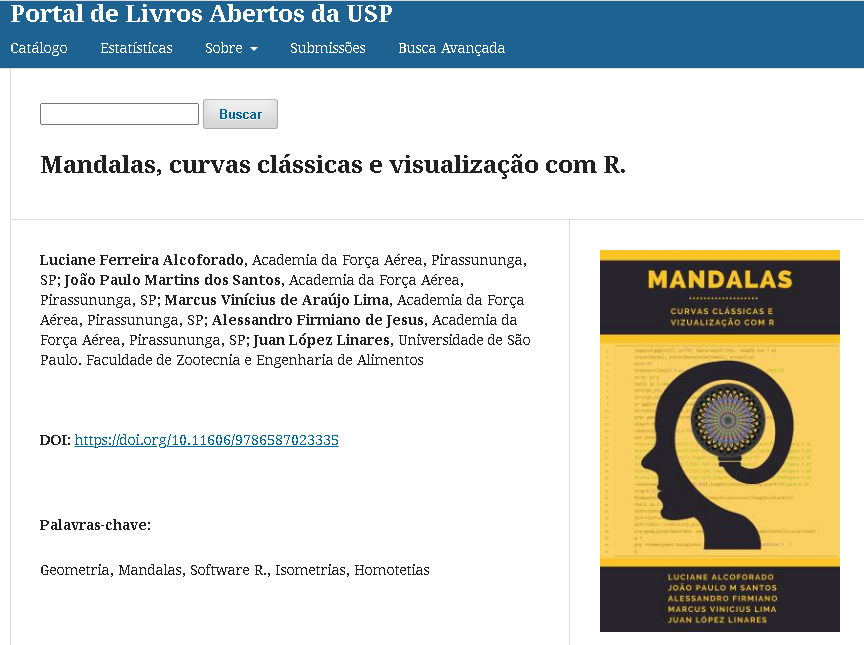
\includegraphics[width=1.5625in,height=\textheight]{FigurasLatinR2023/FigLivro01.png}

}

\end{figure}
\end{frame}

\begin{frame}{Pacote R: mandalaR}
\protect\hypertarget{pacote-r-mandalar}{}
\url{https://cran.r-project.org/web/packages/MandalaR/index.html}

\begin{itemize}
\item
  Genera mandalas a partir de la selección de un conjunto de curvas
  clásicas.
\item
  un método con elección del ángulo de rotación y 3 pasos de traslación
  fijos
\item
  Necesidad de desarrollar nuevas funciones.
\end{itemize}

\begin{figure}

{\centering 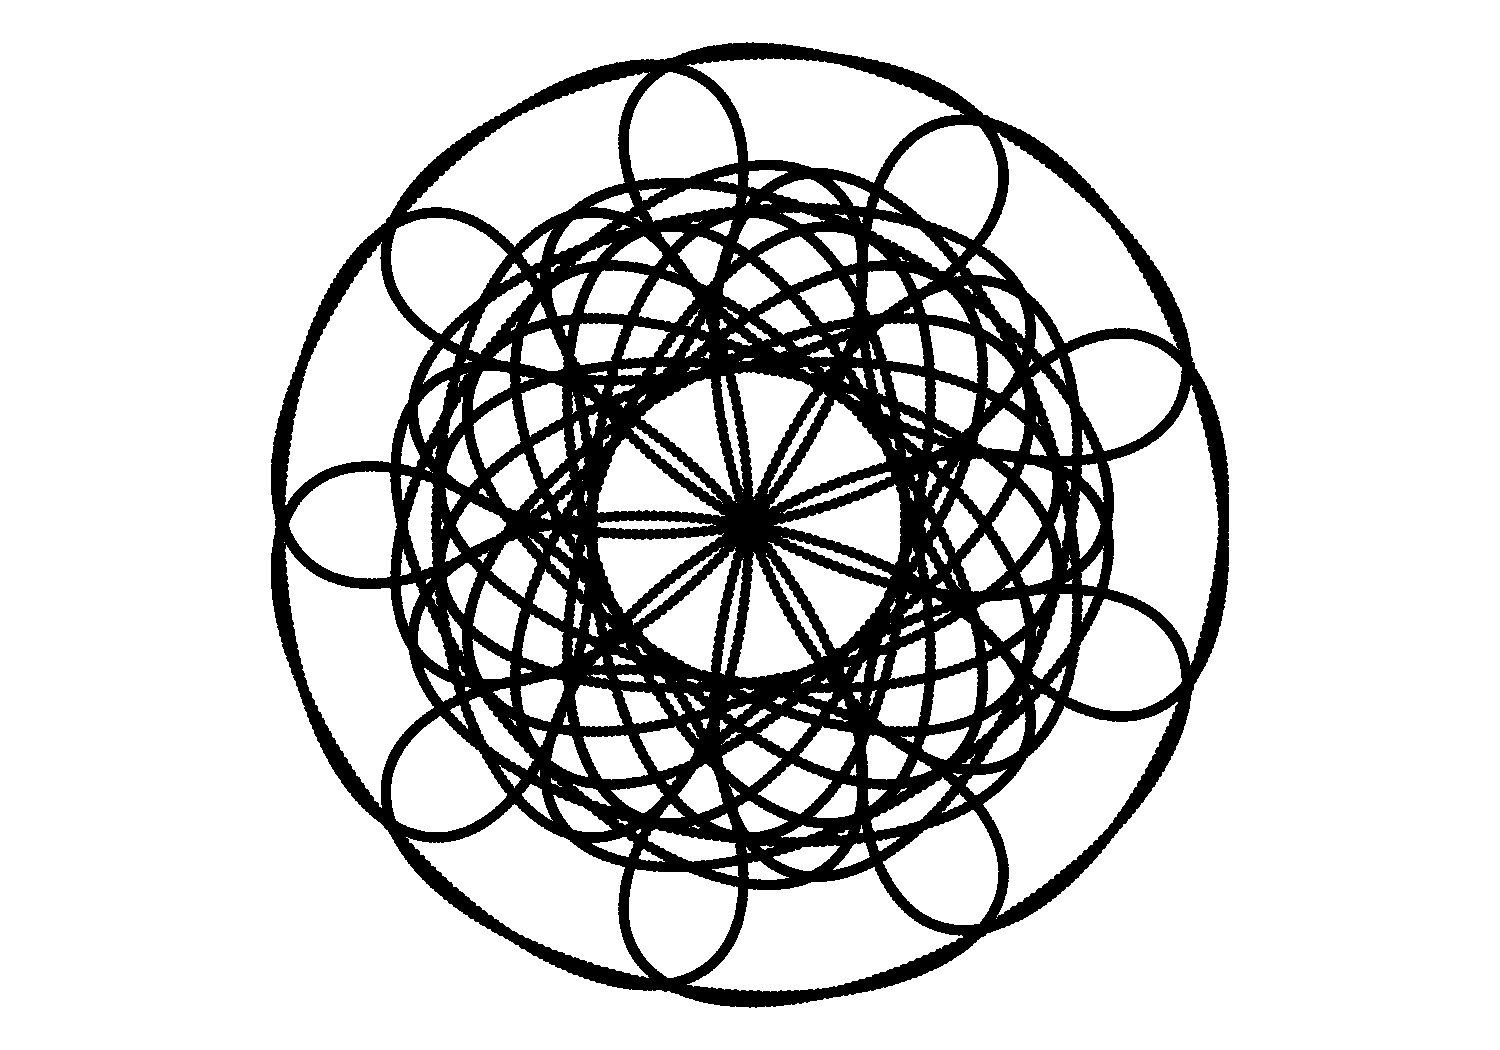
\includegraphics[width=1.875in,height=\textheight]{Teste_quarto_files/figure-beamer/unnamed-chunk-6-1.pdf}

}

\end{figure}
\end{frame}

\begin{frame}{Aplicativo shiny}
\protect\hypertarget{aplicativo-shiny}{}
\begin{itemize}
\item
  Precursor del paquete MandalaR
\item
  Permite generar mandalas sin esfuerzo de programación
\end{itemize}

\begin{figure}

{\centering 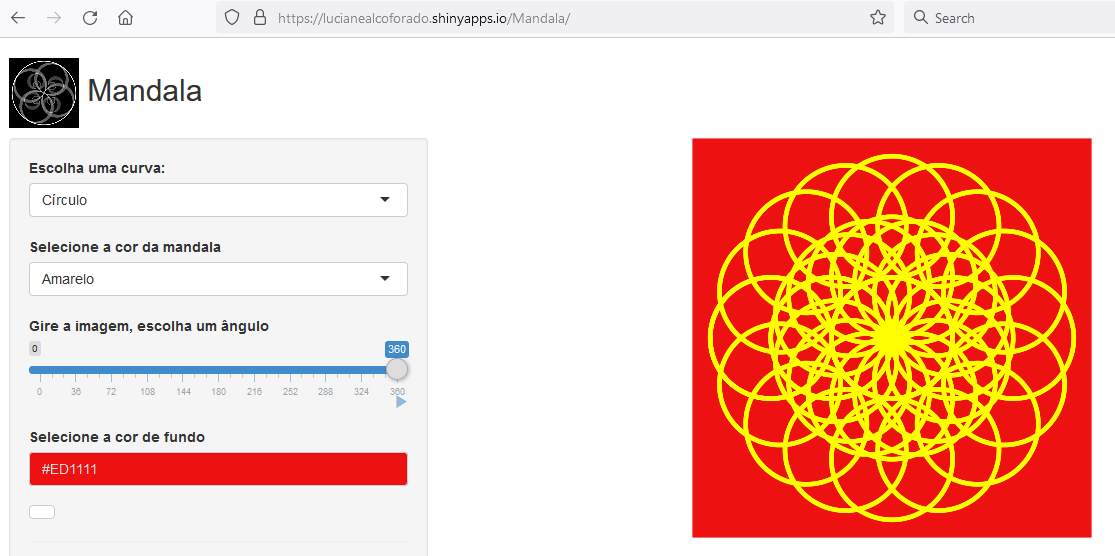
\includegraphics{FigurasLatinR2023/shiny_mandala.png}

}

\caption{https://lucianealcoforado.shinyapps.io/Mandala/}

\end{figure}
\end{frame}

\begin{frame}{Introducción}
\protect\hypertarget{introducciuxf3n}{}
\begin{itemize}
\tightlist
\item
  Valores Humanos: respeto a la diversidad cultural.
\item
  Habilidades Humanas: creatividad, concentración, razonamiento lógico
\item
  Actividades que incluyen R
\item
  Mándalas
\end{itemize}
\end{frame}

\begin{frame}{Objetivo}
\protect\hypertarget{objetivo}{}
\begin{itemize}
\tightlist
\item
  Estimular el aprendizaje y uso del lenguaje R de manera innovador
\end{itemize}

\textrm{\large{R + Matemáticas + Arte = Mándalas}}
\end{frame}

\begin{frame}[fragile]{Paquetes Requeridos para la Actividad}
\protect\hypertarget{paquetes-requeridos-para-la-actividad}{}
\begin{itemize}
\tightlist
\item
  \textbf{ggplot2} y \textbf{mandalaR}
\end{itemize}

\begin{Shaded}
\begin{Highlighting}[]
    \FunctionTok{install.packages}\NormalTok{(}\StringTok{"MandalaR"}\NormalTok{)}
    \FunctionTok{install.packages}\NormalTok{(}\StringTok{"ggplot2"}\NormalTok{)}
\end{Highlighting}
\end{Shaded}
\end{frame}

\begin{frame}{Mandalas}
\protect\hypertarget{mandalas}{}
La relación entre el Mandala y las matemáticas se encuentra en su
significado (círculo). Los mandalas están compuestos por figuras
geométricas que se repiten mediante transformaciones matemáticas.
Además, los mandalas aparecen en diferentes culturas.

\textbackslash begin\{minipage\}\{.9\textwidth\} \center

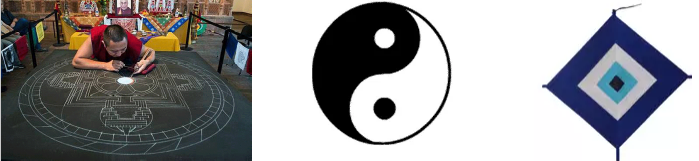
\includegraphics[width=1\textwidth,height=\textheight]{FigurasLatinR2023/culturas_mandalas.png}

\textbackslash end\{minipage\}
\end{frame}

\begin{frame}{Explorando conceptos matematicos - circunferencia}
\protect\hypertarget{explorando-conceptos-matematicos---circunferencia}{}
\begin{figure}

{\centering 
\includegraphics[width=0.52083in,height=\textheight]{FigurasLatinR2023/Circulo.png}

}

\end{figure}

\begin{itemize}
\item
  Fundamental para el estudio de curvas clásicas.
\item
  Ecuación paramétrica:
\end{itemize}

\(x=r\cos(\theta)\)

\(y=r\sin(\theta)\)

\(\theta\in [0,2\pi]\)
\end{frame}

\begin{frame}[fragile]{Circunferencia: código R}
\protect\hypertarget{circunferencia-cuxf3digo-r}{}
\begin{Shaded}
\begin{Highlighting}[]
    \FunctionTok{require}\NormalTok{(ggplot2)}
\NormalTok{    n}\OtherTok{=}\DecValTok{500}
\NormalTok{    t}\OtherTok{=}\FunctionTok{seq}\NormalTok{(}\DecValTok{0}\NormalTok{,}\DecValTok{2}\SpecialCharTok{*}\NormalTok{pi, }\AttributeTok{length.out =}\NormalTok{ n)}
\NormalTok{    raio}\OtherTok{=}\DecValTok{1}
\NormalTok{    x}\OtherTok{=}\NormalTok{raio}\SpecialCharTok{*}\FunctionTok{cos}\NormalTok{(t)}
\NormalTok{    y}\OtherTok{=}\NormalTok{raio}\SpecialCharTok{*}\FunctionTok{sin}\NormalTok{(t)}
\NormalTok{    dt}\OtherTok{=}\NormalTok{tibble}\SpecialCharTok{::}\FunctionTok{tibble}\NormalTok{(x,y)}
\NormalTok{    p}\OtherTok{=}\FunctionTok{ggplot}\NormalTok{()}\SpecialCharTok{+}\FunctionTok{coord\_fixed}\NormalTok{()}\SpecialCharTok{+}\FunctionTok{theme\_void}\NormalTok{();}
\NormalTok{    size}\OtherTok{=}\FloatTok{0.15}
\NormalTok{    p}\OtherTok{=}\NormalTok{p}\SpecialCharTok{+} \FunctionTok{geom\_point}\NormalTok{(}\AttributeTok{data=}\NormalTok{dt, }\FunctionTok{aes}\NormalTok{(}\AttributeTok{x=}\NormalTok{x, }\AttributeTok{y=}\NormalTok{y),}
                    \AttributeTok{color=}\StringTok{\textquotesingle{}black\textquotesingle{}}\NormalTok{,}\AttributeTok{size=}\NormalTok{size)}
\end{Highlighting}
\end{Shaded}
\end{frame}

\begin{frame}[fragile]{Visualización}
\protect\hypertarget{visualizaciuxf3n}{}
\begin{Shaded}
\begin{Highlighting}[]
\NormalTok{p}
\end{Highlighting}
\end{Shaded}

\begin{figure}

{\centering 
\includegraphics[width=2.60417in,height=\textheight]{Teste_quarto_files/figure-beamer/unnamed-chunk-10-1.pdf}

}

\end{figure}
\end{frame}

\begin{frame}{Explorando conceptos matemáticos - Astróide}
\protect\hypertarget{explorando-conceptos-matemuxe1ticos---astruxf3ide}{}
\begin{figure}

{\centering 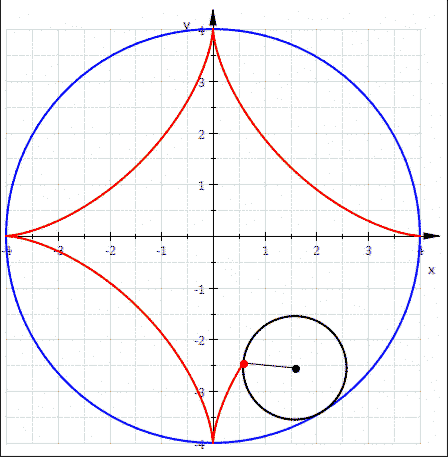
\includegraphics[width=0.83333in,height=\textheight]{FigurasLatinR2023/astroide_circle.png}

}

\end{figure}

\begin{itemize}
\item
  Curva menos conhecida
\item
  Equação paramétrica:
\end{itemize}

\(x=a\cos^3(\theta)\)

\(y=a\sin^3(\theta)\)

\(\theta\in [0,2\pi]\)
\end{frame}

\begin{frame}[fragile]{Astróide: código R}
\protect\hypertarget{astruxf3ide-cuxf3digo-r}{}
\begin{Shaded}
\begin{Highlighting}[]
    \FunctionTok{require}\NormalTok{(ggplot2)}
\NormalTok{    n}\OtherTok{=}\DecValTok{500}
\NormalTok{    t}\OtherTok{=}\FunctionTok{seq}\NormalTok{(}\DecValTok{0}\NormalTok{,}\DecValTok{2}\SpecialCharTok{*}\NormalTok{pi, }\AttributeTok{length.out =}\NormalTok{ n)}
\NormalTok{    a}\OtherTok{=}\DecValTok{1}
\NormalTok{    x}\OtherTok{=}\NormalTok{a}\SpecialCharTok{*}\FunctionTok{cos}\NormalTok{(t)}\SpecialCharTok{\^{}}\DecValTok{3}
\NormalTok{    y}\OtherTok{=}\NormalTok{a}\SpecialCharTok{*}\FunctionTok{sin}\NormalTok{(t)}\SpecialCharTok{\^{}}\DecValTok{3}
\NormalTok{    dt}\OtherTok{=}\NormalTok{tibble}\SpecialCharTok{::}\FunctionTok{tibble}\NormalTok{(x,y)}
\NormalTok{    p}\OtherTok{=}\FunctionTok{ggplot}\NormalTok{()}\SpecialCharTok{+}\FunctionTok{coord\_fixed}\NormalTok{()}\SpecialCharTok{+}\FunctionTok{theme\_void}\NormalTok{();}
\NormalTok{    size}\OtherTok{=}\FloatTok{0.15}
\NormalTok{    p}\OtherTok{=}\NormalTok{p}\SpecialCharTok{+} \FunctionTok{geom\_point}\NormalTok{(}\AttributeTok{data=}\NormalTok{dt, }\FunctionTok{aes}\NormalTok{(}\AttributeTok{x=}\NormalTok{x, }\AttributeTok{y=}\NormalTok{y),}
                    \AttributeTok{color=}\StringTok{\textquotesingle{}black\textquotesingle{}}\NormalTok{,}\AttributeTok{size=}\NormalTok{size)}
\end{Highlighting}
\end{Shaded}
\end{frame}

\begin{frame}{Visualización}
\protect\hypertarget{visualizaciuxf3n-1}{}
\begin{figure}

{\centering 
\includegraphics[width=2.60417in,height=\textheight]{Teste_quarto_files/figure-beamer/unnamed-chunk-14-1.pdf}

}

\end{figure}
\end{frame}

\begin{frame}{Transformaciones geométricas: Isometría}
\protect\hypertarget{transformaciones-geomuxe9tricas-isometruxeda}{}
\begin{itemize}
\tightlist
\item
  rotación
\end{itemize}

girar alrededor de un eje

\begin{figure}

{\centering 
\includegraphics{Teste_quarto_files/figure-beamer/unnamed-chunk-16-1.pdf}

}

\end{figure}
\end{frame}

\begin{frame}{Transformaciones geométricas: Isometría}
\protect\hypertarget{transformaciones-geomuxe9tricas-isometruxeda-1}{}
\begin{itemize}
\tightlist
\item
  traslación
\end{itemize}

cambiar la posición del objeto

\begin{figure}

{\centering 
\includegraphics{Teste_quarto_files/figure-beamer/unnamed-chunk-18-1.pdf}

}

\end{figure}
\end{frame}

\begin{frame}{Transformaciones geométricas}
\protect\hypertarget{transformaciones-geomuxe9tricas}{}
\begin{itemize}
\tightlist
\item
  Homotecia: disminuir
\end{itemize}
\end{frame}

\begin{frame}[fragile]{MandalaR}
\protect\hypertarget{mandalar}{}
\begin{itemize}
\tightlist
\item
  Elección de rotación, disminución estandarizada en 3 niveles.
\end{itemize}

\begin{Shaded}
\begin{Highlighting}[]
\FunctionTok{require}\NormalTok{(MandalaR)}
\FunctionTok{mandalar\_basic}\NormalTok{(}\StringTok{"circle"}\NormalTok{, }\AttributeTok{theta =} \FunctionTok{c}\NormalTok{(}\DecValTok{0}\NormalTok{,}\DecValTok{2}\SpecialCharTok{*}\NormalTok{pi), }\AttributeTok{raio=}\DecValTok{1}\NormalTok{, }\AttributeTok{k =} \DecValTok{45}\NormalTok{, }\AttributeTok{n=}\DecValTok{100}\NormalTok{)}
\end{Highlighting}
\end{Shaded}

\begin{figure}

{\centering 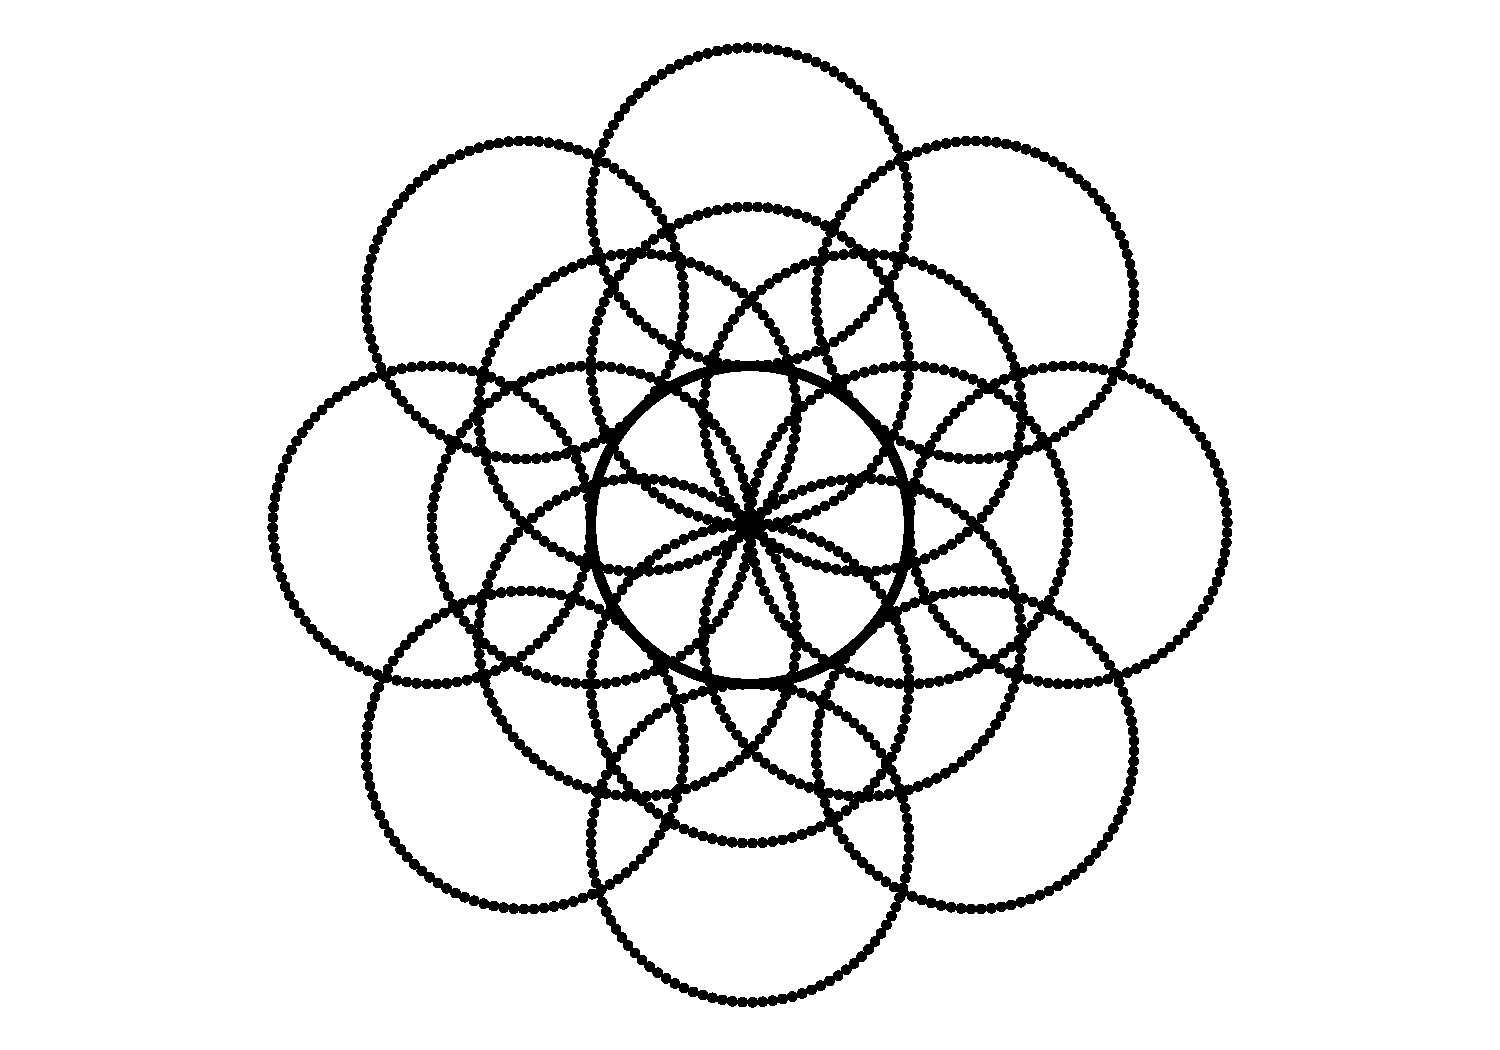
\includegraphics[width=2.60417in,height=\textheight]{Teste_quarto_files/figure-beamer/unnamed-chunk-21-1.pdf}

}

\end{figure}

\begin{itemize}
\tightlist
\item
  cambiando la rotación
\end{itemize}

\begin{Shaded}
\begin{Highlighting}[]
\FunctionTok{mandalar\_basic}\NormalTok{(}\StringTok{"circle"}\NormalTok{, }\AttributeTok{theta =} \FunctionTok{c}\NormalTok{(}\DecValTok{0}\NormalTok{,}\DecValTok{2}\SpecialCharTok{*}\NormalTok{pi), }\AttributeTok{raio=}\DecValTok{1}\NormalTok{, }\AttributeTok{k =} \DecValTok{90}\NormalTok{, }\AttributeTok{n=}\DecValTok{100}\NormalTok{)}
\end{Highlighting}
\end{Shaded}

\begin{figure}

{\centering 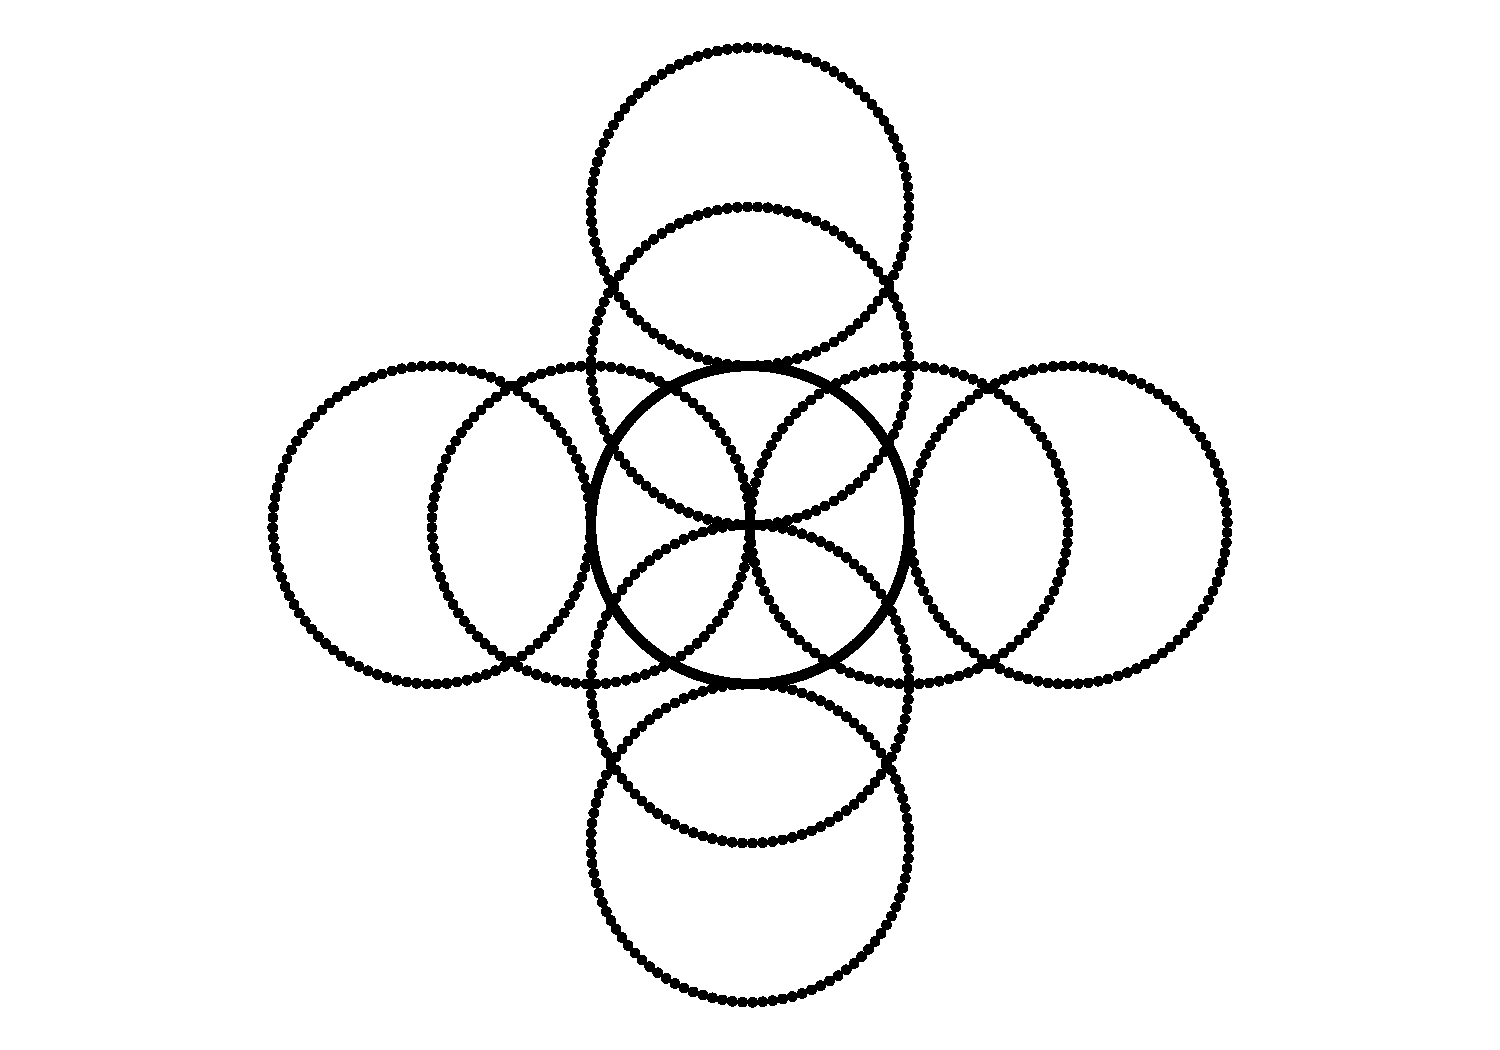
\includegraphics[width=2.60417in,height=\textheight]{Teste_quarto_files/figure-beamer/unnamed-chunk-22-1.pdf}

}

\end{figure}
\end{frame}

\begin{frame}{Coloreando a mano}
\protect\hypertarget{coloreando-a-mano}{}
Desarrolla la atención y la concentración, la motricidad fina, la
creatividad y la imaginación, el sentido estético.

\begin{itemize}
\tightlist
\item
  impresión en papel y pintura a mano
\end{itemize}

inserir exemplos
\end{frame}

\begin{frame}{Coloreando con R}
\protect\hypertarget{coloreando-con-r}{}
Desarrolla la capacidad de lógica matemática y programación.

\begin{itemize}
\tightlist
\item
  uso de la lógica de programación
\end{itemize}
\end{frame}

\begin{frame}{Historia del Arte}
\protect\hypertarget{historia-del-arte}{}
Respetar la diversidad cultural, entendiendo los significados simbólicos
y religiosos de cada tradición.
\end{frame}

\begin{frame}{Referências}
\protect\hypertarget{referuxeancias}{}
\tiny
\end{frame}

\begin{frame}{Obrigado!}
\protect\hypertarget{obrigado}{}
\begin{itemize}
\tightlist
\item
  contato: email aqui!
\end{itemize}
\end{frame}



\end{document}
